
\documentclass[12pt,a4paper]{article}
\usepackage[english]{babel}
\usepackage[utf8]{inputenc}
% \usepackage[utf8]{vietnam}
\usepackage{amsmath}
\usepackage{amsfonts}
\usepackage{authblk}
\usepackage{graphicx} % Required for including images
\usepackage{subcaption} % For subfigures
\usepackage{hyperref} % Add this line at the top with other \usepackage commands
\usepackage{cite}
\usepackage{tikz}
\usetikzlibrary{shadows,arrows.meta,positioning}

\title{Variable Impedance Actuators: a Review}
\author[1,2]{Do Thanh Trung}
\author[2]{N MH}
\affil[1]{\textit{HELLA VIETNAM}}
\affil[2]{\textit{HCM UTE, \href{https://www.hcmute.edu.vn}
        {\texttt
            {
                \fontfamily{pcr}\selectfont www.hcmute.edu.vn
            }
        }
    }
}
\date{\today}

\begin{document}
    \maketitle
    \noindent\rule{\textwidth}{0.4pt}
    \begin{abstract}
        Variable Impedance Actuators (VIA) have received increasing attentionin recent years as many novel applications involving interactions with an un-known and dynamic environment including humans require actuators withdynamics that are not well-achieved by classical stiffactuators. This paperpresents an overview of the different VIAs developed and proposes a clas-sification based on the principles through which the variable stiffness anddamping are achieved. The main classes are active impedance by control,inherent compliance and damping actuators, inertial actuators, and combi-nations of them, which are then further divided into subclasses. This classi-fication allows for designers of new devices to orientate and take inspirationand users of VIA’s to be guided in the design and implementation processfor their targeted application.
        
    \end{abstract}
    \textit{Keywords}: Variable Impedance Actuators, Variable Stiffness Actuators, Variable Damping Actuators, Compliant Actuators
    
    \noindent\rule{\textwidth}{0.4pt}
    \section{Introduction}
    Actuators are key enabling components for motion generation and controlwith properties that greatly impact the overall performance of any mechan-ical systems. The lack of suitable actuators has hindered the developmentof high performance machines with capabilities comparable to humans, espe-cially with respect to motion, safety and energy efficiency of human or otheranimals. The functional and neuro-mechanical control performances of bio-Preprint submitted to Robotics and Autonomous Systems June 17, 2013*ManuscriptClick here to view linked Referenceslogical muscle far exceeds that of mechanical devices, with a key differencebeing the adaptable compliance or variable stiffness found in biological sys-tems; this is very different from the performance of traditional stiffelectricaldrives used in industrial robotics, which require accurate, reference-trajectorytracking. Recent applications such as robots in close human/robot proxim-ity, legged autonomous robots, and rehabilitation devices and prostheses, setdifferent design specifications, where compliant actuators can have signifi-cant advantages over traditional actuation. Variable Impedance Actuators(VIA) are rapidly developing with a wide range of different actuators basedon different principles, but as yet there is not “winning” design. Indeed,probably there is no winning actuator, but rather application dependent op-timal solutions. To understand this “zoology”, the VIACTORS consortium \cite{RN283} provides in this paper an overview as well as a categorization, discussingadvantages and disadvantages of the different designs. This work is the firstof three papers on VIAs, which tries to organize the VIA state of the art,and establish a common language for designers and potential users of VIAtechnology. Grioli et al. \cite{RN280} present a Variable Stiffness Actuator (VSA)datasheet as an interface language between designers and users and discussdesign procedures and how data generic VSA data may be organized to min-imize the engineer’s effort in choosing the actuator type and size. Wolf etal. [3] propose VSA Design Guidelines for R\&D engineers facing the chal-lenge of designing new VSA systems and implementing them in use-cases asshock absorbing, stiffness variation, cyclic motions and explosive motions.The development and exploitation of novel actuation technologies will cre-ate a new generation of robots that can co-exist and co-operate with peopleand get much closer to the human levels of manipulation, locomotion andrehabilitation performances.

    \section{Classification of Variable Impedance Actuators}
    Position control in a task in which a robot interacts with the environ-ment, is not a properly posed problem because the controller is dependenton parameters, which are out of the control potential. Yet, controllingthe impedance and the equilibrium position is a well-posed problem that isindependent of the knowledge of the environment, if within certain bound-aries. Applications of VIA are consequently found were robots must phys-ically interact with an unknown and dynamic environment and the controlbody-actuator system must have abilities like :
    \begin{itemize}
        \item Efficiency e.g. natural gait generation, adaptation in legged locomotionand prosthetics for lower limbs, explosive motions such as throwing orkicking;
        \item Robustness to external perturbations and unpredictable model errors(changes) of the environment, of the robot kinematics and dynamics,or of the dynamics of a human interacting with it;
        \item Adaptability and force accuracy in the interaction with the operator, inapplications in which continuous contact and accurate force exchangeis necessary, such as in “hands-on” assistive devices, rehabilitation, ex-oskeletons and haptics;
        \item Safety to humans (and resilience to self-damage) in operations wherethe robot has fast, accurate motions, while cooperating, physically in-teracting or even possibly colliding with the humans and their environ-ment, including other robots.
    \end{itemize}
    \begin{figure}[ht]
        \centering
        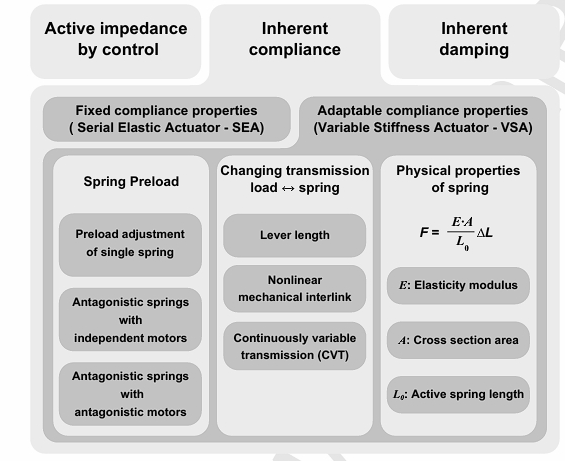
\includegraphics[width=0.7\textwidth]{figures/fig1.png}
        \caption{HELLO WORLD}\label{fig:HELLO_WORLD}
    \end{figure}

    \begin{figure}[ht]
        \centering
        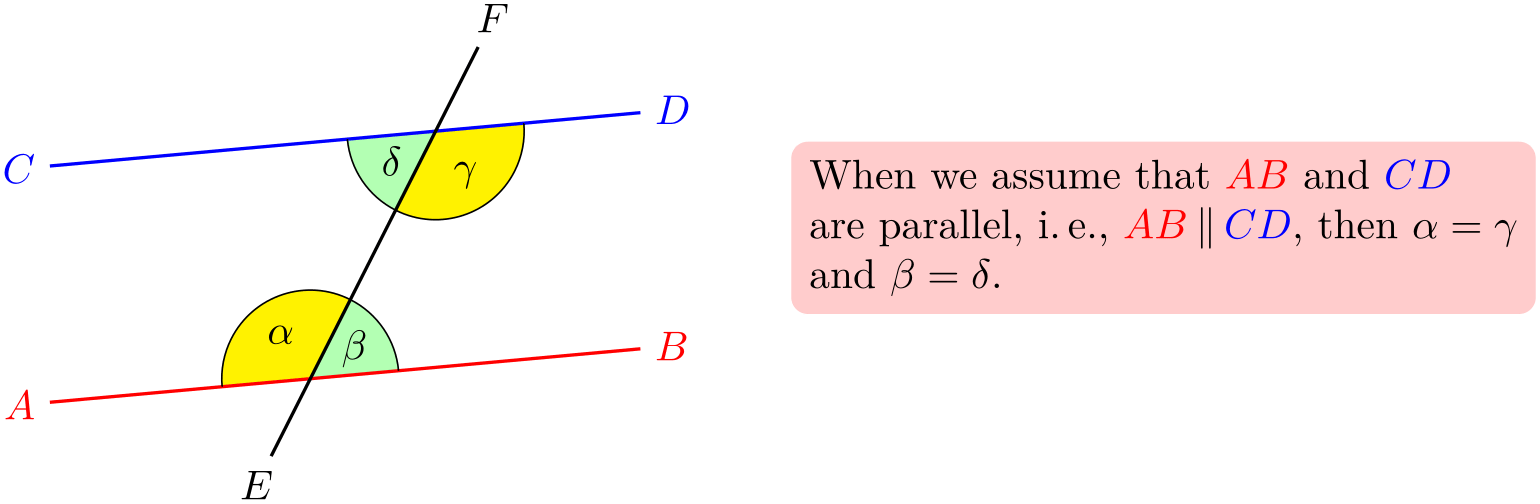
\includegraphics[width=0.7\textwidth]{figures/fig2.png}
        \caption{Overview of Variable Impedance Actuator classification.}
        \label{fig:VIA_classification}
    \end{figure}

    The main classes of VIA are active impedance by control,
    inherent com-pliance and damping actuators, inertial actuators,
    and combinations of them, which are then further divided into subclasses 
    as shown in Fig.\ref{fig:VIA_classification}.

        \begin{figure}
            \centering
                \begin{subfigure}{0.45\textwidth}
                    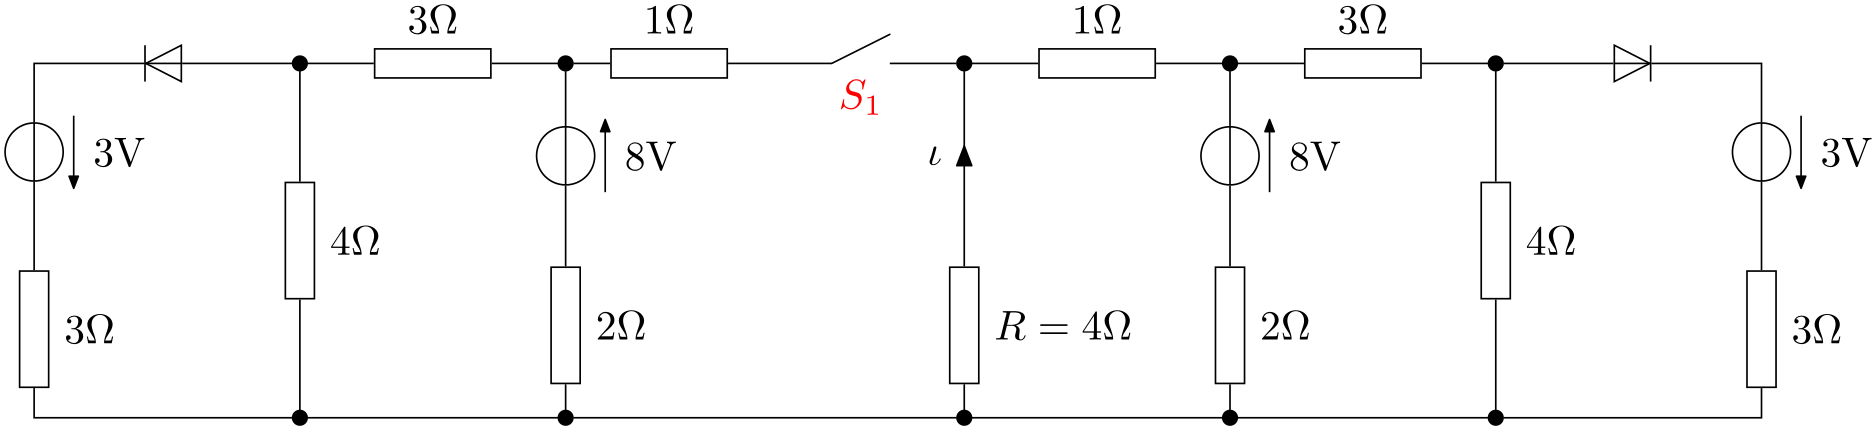
\includegraphics[width=0.7\textwidth]{figures/fig5.png}
                    \caption{Schematic of a general VIA.}
                    \label{fig:a_general_VIA}
                \end{subfigure}
                \hfill
                \begin{subfigure}{0.45\textwidth}
                    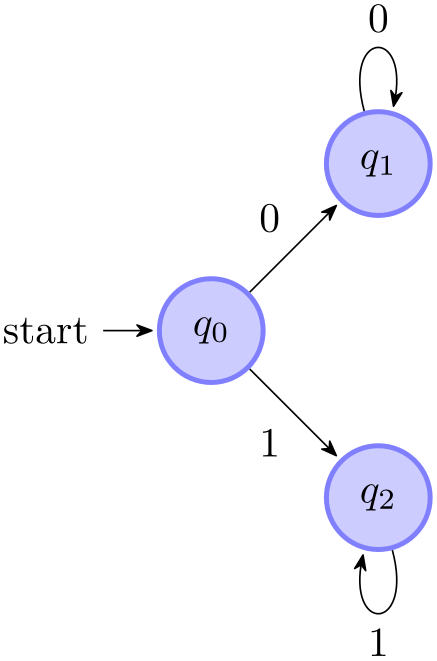
\includegraphics[width=\textwidth]{figures/fig4.png}
                    \caption{Series Elastic Actuator (SEA).}\label{fig:b_general_VIA}
                \end{subfigure}
            \caption{Schematic of a general VIA.}\label{fig:general_VIA}
        \end{figure}
    
    A general VIA is schematically shown in Fig.\ref{fig:a_general_VIA}, where the motor drives the load through a transmission and a variable impedance element. The motor can be controlled in position, velocity, torque or impedance. The variable impedance element can be a spring and/or a damper, whose mechanical properties can be changed by an additional mechanism. The load can be a link of a robot or any other mechanical system. A typical example of a VIA is the Series Elastic Actuator (SEA) shown in Fig.\ref{fig:b_general_VIA}, where the motor drives the load through a transmission and an elastic element (spring). The motor is usually controlled in position or velocity, while the torque applied to the load is measured by measuring the deflection of the spring. The stiffness of the spring is fixed and cannot be changed during operation. However, by controlling the motor position, the equilibrium position of the spring can be changed, thus changing the effective stiffness of the actuator at low frequencies. SEAs have been widely used in various applications, such as legged robots, prosthetics, and exoskeletons, due to their inherent compliance and ability to store and release energy.

    \section{Principles of Variable Stiffness}
    Several groups have designed adaptable compliance mechanisms, with
    elastic elements storing energy, in addition to altering the stiffness. This
    concept gives intrinsic capabilities (bandwidth, impacts, energy storage) over
    the joint stiffness range. However, two motors are required: one to control
    the equilibrium position and the second to control stiffness. In this section, a
    classification is presented, based on the main principle on which the adaptive
    stiffness is obtained (see Fig. 2). The different actuators from literature can
    be classified into three major groups:
    \begin{itemize}
        \item \textbf{Spring Preload}: Stiffness is altered by changing the spring preload.
        \item \textbf{Changing transmission between load and spring}: The stiffness 
        is altered by changing the transmission ratio between the output link
        and the elastic elements.
        \item \textbf{Physical properties of the spring}: The physical structure of the
        \item \bfseries The physical structure of the
        spring itself is altered.
    \end{itemize}

    Some devices use combinations of these main three mechanical properties.
    \usetikzlibrary {angles,calc,quotes}
    \begin{tikzpicture}[angle radius=.75cm]

        \node (A) at (-2,0)     [red,left]   {$A$};
        \node (B) at ( 3,.5)    [red,right]  {$B$};
        \node (C) at (-2,2)     [blue,left]  {$C$};
        \node (D) at ( 3,2.5)   [blue,right] {$D$};
        \node (E) at (60:-5mm)  [below]      {$E$};
        \node (F) at (60:3.5cm) [above]      {$F$};

        \coordinate (X) at (intersection cs:first line={(A)--(B)}, second line={(E)--(F)});
        \coordinate (Y) at (intersection cs:first line={(C)--(D)}, second line={(E)--(F)});

        \path
            (A) edge [red, thick]  (B)
            (C) edge [blue, thick] (D)
            (E) edge [thick]       (F)
            pic ["$\alpha$", draw, fill=yellow]   {angle = F--X--A}
            pic ["$\beta$",  draw, fill=green!30] {angle = B--X--F}
            pic ["$\gamma$", draw, fill=yellow]   {angle = E--Y--D}
            pic ["$\delta$", draw, fill=green!30] {angle = C--Y--E};

        \node at ($ (D)!.5!(B) $) [right=1cm,text width=6cm,rounded corners,fill=red!20,inner sep=1ex]
            {
            When we assume that $\color{red}AB$ and $\color{blue}CD$ are
            parallel, i.\,e., ${\color{red}AB} \mathbin{\|} \color{blue}CD$,
            then $\alpha = \gamma$ and $\beta = \delta$.
            };
    \end{tikzpicture}

    \section{Principles of Variable Damping}

    \section{Active Impedance Control}

    \section{Inherent Compliance and Damping Actuators}

    \section{Inertial Actuators}

    \section{Combined Approaches}

    \section{Design Guidelines}

    \section{Applications}

    \section{Conclusion}

    \section*{References}
    % \begin{thebibliography}{00}
        
    %     \bibitem{b1} VIACTORS Consortium, "Variable Impedance Actuators for Compliant and Agile Robots", EU FP7 ICT-2011.4.3, Project No. 287894, 2012-2015.
        
    %     \bibitem{b2} Grioli, G., Catalano, M., Garabini, M., and Bicchi, A. (2012). "A data sheet for variable stiffness actuators". IEEE Robotics \& Automation Magazine, 19(3), 20-32.
        
    %     \bibitem{b3} Wolf, S., Albu-Schäffer, A., and Hirzinger, G. (2011). "A new variable stiffness design: Matching requirements of the next robot generation". In 2011 IEEE International Conference on Robotics and Automation (pp. 1741-1746). IEEE.
    % \end{thebibliography}
    \bibliographystyle{IEEEtran}
    \bibliography{EVALUATION_CITE}

\end{document}
